\section{Methodology}
\hide{
\begin{table}[]
    \caption{Notation Description}
    \centering
    \begin{tabular}{c|c}
    \hline
       $\mathbf{X}_{\alpha}$  & activity feature \\ \hline
       $\mathbf{X}_{\alpha}^{(i)}$ & $i^{th}$ feature group of activity feature \\ \hline
       $\mathbf{X}_{\beta}$  & user-specific feature \\ \hline
       $\mathbf{X}_{\gamma}$   & course-specific feature \\ \hline
       $\textbf{E}^{(i)}_\alpha$ & embedding of $\mathbf{X}_{\alpha}^{(i)}$ \\ \hline
       $\mathbf{E}_\beta$ & embedding of   $\mathbf{X}_{\beta}$ \\ \hline
        $\mathbf{E}_\gamma$ & embedding of   $\mathbf{X}_{\gamma}$ \\ \hline
         $\textbf{V}_\alpha$ &  activity feature maps \\ \hline
       $\mathbf{V}_\beta$ & user-specific feature map \\ \hline
        $\mathbf{V}_\gamma$ & course-specific feature map\\ \hline
    \end{tabular}
    \label{tab:my_label}
\end{table}
}
We now turn to discuss potential solutions to predict when and whether a user will drop out a specific course, 
by leveraging the patterns discovered in the above analysis. In summary, we propose a Context-aware Feature Interaction Network (\modelname{}) to deal with the dropout prediction problem. Different from previous work on this task, the proposed model incorporates context information, including user and course information, into a unified framework. Let us begin with a formulation of the problem we are going to address.

\subsection{Formulation}
	\label{ProblemDef}
	

\begin{figure}
	\centering
	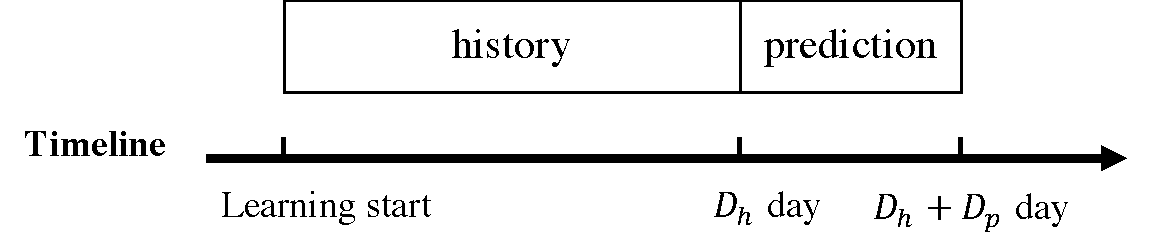
\includegraphics[width=0.8\linewidth]{course-span.pdf}
	
	\caption{Dropout Prediction Problem. The first $D_h$ days are \emph{history period}, and the next $D_p$ days are \emph{prediction period}.}
	\label{fig:dataCons}
\end{figure}
\hide{
	\item{Activity Count/Ratio:} For each enrollment $(u,c)$, we calculate the number and ratio for each type of activities in table \ref{ResourceAction}. 
\item{Activity Temporal Statistics:} The whole duration time of a course is divided by weeks, and the activity counts and statistics(including \emph{max, min, stdev, median}) in different weeks are used as features.
\item{Activity Count in Hours Per Day:} We calculate user activity count for each hour in a day (24 hours).
\item{Activity Count in Day Per Week:} We compute user activity count for each day in a week (5 weekdays + 2 weekends).
\item{Activity N-gram Count/Ratio:} The N-grams of activity sequence is used to capture the correlations between neighbor activities. We employ N-gram activity count and ratio as the N-gram features.
\item{Engagement Style:} Following the taxonomy of engagement introduced by Anderson et al. \cite{Anderson:2014:EMO:2566486.2568042ß}, we use the $\emph{assignment fraction} = \frac{ \emph{watching video \#}}{ \emph{complete assignment \#}}$ to represent user's engagement pattern.
\item{Learning Time Span:} A user's learning time span is the duration between a user's first visit time and her last visit time on a course.  

\item{Effective Learning Time:} The \emph{effective learning time} introduced by Qiu et al. \cite{Qiu:2016:MPL:2835776.2835842} is an approximated method to compute user's actual study time on a certain course. This is calculated based on the time interval between user's \emph{watching video} and \emph{stop video}, and we employ this feature in our paper.

\item{Visiting Time Interval:} A user's interval time for visiting one course reflects user's interests in this course. The statistics(\emph{max, min, stdev, median}) of visiting time intervals are used as features.\\
}
\hide{
\begin{table*}[]
	\caption{Activity Features}
	\centering
	\begin{tabular}{p{3.7cm}|p{13.4cm}}
		\hline
		Activity Count/Ratio  &  Total number and ratio of each type of learning activities\\ \hline
		Activity Temporal Statistics&  The whole duration time of a course is divided by weeks, and the activity counts and statistics(including \emph{max, min, stdev, median}) in different weeks are used as features.\\ \hline
		Activity Count Per Hour  &  The number of users' learning activities for each hour in a day (24 hours).\\ \hline
		Activity Count Per Day & The number of users' learning activities for each day in a week (5 weekdays + 2 weekends). \\ \hline
		Activity N-gram Count/Ratio & The N-grams of activity sequence is used to capture the correlations between neighbor activities. We employ N-gram activity count and ratio as the N-gram features. \\ 
	 \hline
		Engagement Style & Following the taxonomy of engagement introduced by Anderson et al. \cite{Anderson:2014:EMO:2566486.2568042ß}, we use the $\emph{assignment fraction} = \frac{ \emph{watching video \#}}{ \emph{complete assignment \#}}$ to represent user's engagement pattern.  \\ \hline
		Learning Time Span & A user's learning time span is the duration between a user's first visit time and her last visit time on a course.  \\ \hline
		Effective Learning Time & The \emph{effective learning time} introduced by Qiu et al. \cite{Qiu:2016:MPL:2835776.2835842} is an approximated method to compute user's actual study time on a certain course. This is calculated based on the time interval between user's \emph{watching video} and \emph{stop video}, and we employ this feature in our paper.\\ \hline
		Visiting Time Interval & A user's interval time for visiting one course reflects user's interests in this course. The statistics(\emph{max, min, stdev, median}) of visiting time intervals are used as features.
		\\ \hline
	\end{tabular}
	\label{tab:acvtityFeat}
\end{table*}
}
%Our main task is to predict whether a user would dropout from an enrolled course in a pre-specified time window. 
In order to formulate this problem more precisely, we first introduce the following definitions. 

\emph{Definition 2.} \textbf{Enrollment Relation}: Let $\mathbb{C}$ denote the set of courses, $\mathbb{U}$ denote the set of users, and the pair $(u,c)$ denote user $u\in \mathbb{U}$ enrolls the course $c\in \mathbb{C}$.
The set of enrolled courses by $u$ is denoted as  $\mathbb{C}_u\subset \mathbb{C}$ and 
the set of users who have enrolled course $c$ is denoted as $\mathbb{U}_c\subset \mathbb{U}$.
We use $\mathbb{E}$ to denote the set of all enrollments, i.e., $\{(u,c)\}$

\emph{Definition 3.} \textbf{Learning Activity}: 
In MOOCs, user $u$'s learning activities in a course $c$ can be formulated into an $m_x$-dimensional vector $\mathbf{X}(u,c)$, where each element $x_i(u,c) \in \mathbf{X}(u,c)$ is a continuous feature value associated to $u$'s learning activity in a course $c$. Those features are extracted from user historical logs, mainly includes the statistics of users' activities.

\emph{Definition 4.} \textbf{Context Information}: Context information in MOOCs comprises user and course information. User information is represented by user demographics (i.e. gender, age, location, education level) and user cluster. While course information is the course category. The categorical information (e.g. gender, location) is represented by a one-hot vector, while continues information (i.e. age) is represented as the value itself. By concatenating all information representations, the context information of a $(u,c)$ pair is represented by a vector $\mathbf{Z}(u,c)$.   


%Activity pattern vector mainly includes users' learning behavioral features, which are extracted from user historical activity logs. The details are exhibited in Table \ref{tab:acvtityFeat}. User-related pattern vector consists of user demographics (i.e. gender, age, location, education level and user id) and user cluster (Cf. Section \ref{sec:temporal}). Course-related pattern vector,  including course id and course category, is used to represent course specific information in MOOCs. \\
%Specifically the pattern vector includes three types of patterns: activity pattern vector $\mathbf{X}_a \in \mathbb{R}^{m_a}$, user-specific pattern vector $\mathbf{X}_u \in \mathbb{R}^{m_u}$ and course-specific pattern vector $\mathbf{X}_c \in \mathbb{R}^{m_c}$.  

% into a paired tuple  $x = (a, t)$, where $a$ represents user's action(such as ``watching video'') and $t$ is the corresponding logged time stamp. In this paper, we focus on four types of learning activities: \emph{video, forum, assignment, web page}, which are described in table \ref{ResourceAction}. \\

%Each course has a set of available resources for users, such as video and forum. Here we use $R$ to represent the resource set of course on MOOCs. For each resource $r \in R$, there are a set of specific actions for it. We use $A$ to denote the action set. In this paper, we focus on four types of resources on MOOCs: \emph{video, forum, assignment, web page}, which are shown in table \ref{ResourceAction}, together with the corresponding actions. 

%Then a learning activity record of $u\in \mathbb{U}$ in one enrolled course $c\in \mathbb{U}_c$ at time $t$ can be represented as $X=(u,c,r,a,t)$, where $r\in R$ is the resource $u$ has accessed, $a\in A$ is the corresponding action on $r$. For each $(u,c) \in \mathbb{E}$, we use $\mathcal{X}_{uc}$ to represent user $u$'s historical learning activity set on $c$.\\

With these definitions, our problem of dropout prediction can be defined as: Given user $u$'s learning activity $\mathbf{X}(u,c)$ on course $c$ in \textit{history period} (as shown in Figure \ref{fig:dataCons}, it is the first $D_h$ days after the learning starting time), as well as her/his context information $\mathbf{Z}(u,c)$, our goal is to predict whether $u$ will drop out from $c$ in the \textit{prediction period} (as shown in Figure \ref{fig:dataCons}, it is the following $D_p$ days after \textit{history period}). More precisely, let $y_{(u,c)} \in \{0,1\}$ denote the ground truth of whether $u$ has dropped out, $y_{(u,c)}$ is positive if and only if $u$ has not taken activities on $c$ in the \textit{prediction period}. Then our task is to learn a function:
%Given user $u$'s activity sequence $X_{(u,c)}= [x_1, x_2,...,x_N]$ on course $c$ in \textit{history period}(as shown in Figure \ref{fig:dataCons}, it is the first $D_h$ days after the learning starting time), our goal is to predict whether $u$ will drop out from $c$ in the \textit{prediction period}(as shown in Figure \ref{fig:dataCons}, it is the following $D_p$ days after \textit{history period}). More precisely, let $y_{(u,c)} \in \{0,1\}$ denote the ground truth of whether $u$ has dropped out, $y_{(u,c)}$ is positive if and only if $u$ has not taken activities on $c$ in the \textit{prediction period}. Then our task is to learn a function:

$$f: (\mathbf{X}(u,c), \mathbf{Z}(u,c))\to y_{(u,c)}$$ 

\hide{Let $\mathbb{C}$ denote the set of courses, $\mathbb{U}$ denote the set of users, and the pair $(u,c)$ denote user $u\in \mathbb{U}$ enrolls the course $c\in \mathbb{C}$.
The set of enrolled courses by $u$ is denoted as  $\mathbb{C}_u\subset \mathbb{C}$ and 
the set of users who have enrolled course $c$ is denoted as $\mathbb{U}_c\subset \mathbb{U}$.
We use $\mathbb{E}$ to denote the set of all enrollments, i.e., $\{(u,c)\}$.
Given this, our problem of dropout prediction can be defined as:}

\hide{
	   \emph{Definition 2.} \textbf{$t$-Dropout Prediction}: Given all users $\mathbb{U}$'s learning activity $\textbf{X}^t$ in all courses $\mathbb{C}$ before time $t$, our goal is to learn a function $f$ in order to infer
	   $$f: (\mathbb{U},\mathbb{C},\textbf{X}^t)\to \{y^t_{(u,c)}\}$$
	   \noindent where $y_{(u,c)} \in \{0,1\}$ indicates whether user $u$ would drop out ($y=1$) course $c$ 
	   after time $t$ or not. 
}
\hide{
	   sequence $X_{(u,c)}= [x_1, x_2,...,x_N]$ on course $c$ in \textit{history period}(as shown in Figure \ref{fig:dataCons}, it is the first $D_h$ days after the learning starting time), our goal is to predict whether $u$ will drop out from $c$ in the \textit{prediction period}(as shown in Figure \ref{fig:dataCons}, it is the following $D_p$ days after \textit{history period}). More precisely, let $y_{(u,c)} \in \{0,1\}$ denote the ground truth of whether $u$ has dropped out, $y_{(u,c)}$ is positive if and only if $u$ has not taken activities on $c$ in the \textit{prediction period}. Then our task is to learn a function:
	 $$f: (u,c,X_{(u,c)})\to y_{(u,c)}$$
}    

	
\hide{
Based on the analyses in previous section, users' dropout in a course has high correlation with their context(similar courses and friends). How to construct a personalized prediction system for diverse users in MOOCs is a quite difficult problem. In this section, we introduce our methodology of personalized dropout prediction. We consider three types of features, i.e., activity features, user-related features and course-related features, when predicting users' dropout.
}
\hide{
  \begin{table}
	\hspace{-0.01in}
	\centering
	\caption{Average activity feature values on two sample courses --- Conversational English and Data Structure. CAR --- average correct answer ratio. }
	\small
	\label{tab:sample}
	\setlength{\tabcolsep}{1mm}\begin{tabular}{@{}c@{}|l@{}|c|c}
		\hline
		\hline
		Category &  Type   & Conversational English & Data Structure \\
		\hline
		\multirow{3}{*}{video}&  \#watch &74.80 & 32.48\\	
		\cline{2-4}
		& \#stop     &69.53 & 26.14\\
		\cline{2-4}
		& \#jump   &51.18 & 14.38\\
		\hline
		\multirow{2}{*}{forum}&  \#question & 0.049 & 0.038 \\
		\cline{2-4}
		& \#answer &1.10&0.12 \\
		\hline
		\multirow{2}{*}{assignment} & CAR &0.45 & 0.41 \\
		\cline{2-4}
		& \#revise  &0.09& 0.02 \\
		\hline
		\multirow{2}{*}{session}    & seconds &1,715 &714 \\
		\cline{2-4}                
		&  count     &3.61 &8.13 \\  
		\hline
		\multicolumn{2}{c|}{dropout rate} &0.74 &0.73 \\
		\hline	
		\hline
	\end{tabular}
	\normalsize
\end{table}
}

Please note that we define the prediction of dropouts for all users/courses together, as we need to consider the user and course information. 
%In next section, we will explain the details of our solution --- Context-aware Feature Interaction Network --- for this task.


%Another challenge we have to face is how to incorporate the course correlation and friend influence into the prediction. To solve these challenges, we proposed an Attention-based Feature Interaction Network (AFIN) to predict dropout by incorporating users' context information.
\subsection{Context-aware Feature Interaction Network}
 \begin{figure}
	\hspace{-0.1in}
	\centering
	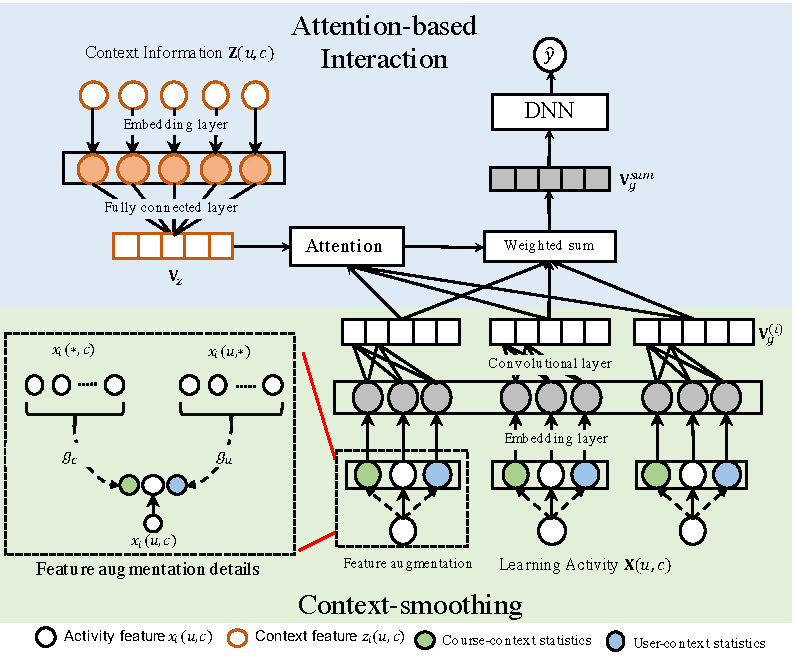
\includegraphics[width=\linewidth]{model_arch_new.pdf}	
	\caption{The architecture of \modelname{}.}
	\label{fig:modelArch}
\end{figure}
\vpara{Motivation.} From prior analyses, we find users' activity patterns in MOOCs have a strong correlation with their context (e.g. course correlation and friends influence). More specifically, the value of learning activity vector $\textbf{X}(u,c)$ is highly sensitive to the context information $\textbf{Z}(u,c)$. 
\hide{
For example, the average activity features of table \ref{tab:sample} presents the average activity feature values of two sample courses of XuetangX (i.e. Conversational English and Data Structure). We observe that these features are totally different between two courses though they have approximate user dropout rates.}
To tackle this issue, we employ convolutional neural networks (CNN) to learn a context-aware representation for each activity feature $x_i(u, c)$ by leveraging its context statistics. This strategy is referred to as context-smoothing in this paper. What's more, we also propose an attention mechanism to learn the importances of different activities by incorporating $\textbf{Z}(u,c)$ into dropout prediction. Figure~\ref{fig:modelArch} shows the architecture of the proposed method.  In the rest of this section, we will explain the context-smoothing and attention mechanism in details.
%However,  very few works have attempted to incorporate the context information into the dropout prediction framework.
% This is the main motivation for our approach. 
 
 %More specifically, we found the value of the learning activity vector $\textbf{X}(u,c)$ is highly sensitive to the context information $\textbf{Z}(u,c)$. Table \ref{tab:sample} presents an example of the average activity feature values on two courses (i.e. Conversational English and Data Structure). We can observe that these features are totally different between two courses though they have a approximate user dropout rate. A general solution for this challenge is to augment the learning activity vector with its statistics of user-level and course-level and feed the augmented learning activity vector into the classifier directly. However, it always suffers from the curse of dimensionality and can not get a better performance. To tackle this issue, we employ convolutional neural networks (CNN) to learn a context-aware representation for each activity feature of $\textbf{X}$ by leveraging its context statistics. This strategy is referred to context-smoothing in this paper. What's more, we also propose an attention mechanism to learn the importances of different activities by incorporating the context information into dropout prediction. Figure~\ref{fig:modelArch} shows the architecture of the proposed method.

%The main technical contributions of Attention-based Feature Interaction Network (AFIN) lies in the proposal of context-smoothing and an attention mechanism to model the correlations among $\mathbf{X}_a$, $\mathbf{X}_u$ and $\mathbf{X}_c$.
%The idea of feature context-smoothing is to augment the context information into each feature and then use convolutional neural networks (CNN) to learn the representation of each feature. We also add an attention layer so as to learn the importances of activity patterns based on user-specific and course-specific patterns.
%In feature augmentation, the learning activity vector $\mathbf{X}$ is expanded with its context statistics. Then each feature and its context statistics are converted into a matrix through an embedding layer, which are integrated into a dense vector by a convolutional neural network in feature fusion step.

\vpara{Context-Smoothing.} %In this section, we will introduce the context-smoothing strategy. 
The context-smoothing strategy consists of three steps: feature augmentation, embedding and feature fusion. 
In feature augmentation, each activity feature $x_i(u,c) \in \textbf{X}(u,c)$\footnote{We ommit the notation $(u,c)$ in the following description, if no ambiguity.} is expanded with its user and course-context statistics. 
User-context statistics of feature $x_i$ is defined by a mapping function $g_u(x_i)$ from the original activity feature to several statistics of $i^{th}$ feature across all courses enrolled by $u$, i.e., 
 $g_u: x_i(u,c) \rightarrow [\text{avg}(\{x_i(u,*)\}), \text{max}(\{x_i(u,*)\}),\ldots]$.
 While course-context statistics, represented by $g_c(x_i)$, are statistics over all users in course $c$, i.e.,
  $g_c: x_i(u,c) \rightarrow [\text{avg}(\{x_i(*,c)\}), \text{max}(\{x_i(*,c)\}),\ldots]$.
  Let  
  $\hat{\mathbf{X}}= \hat{\mathbf{X}}^{(1)}_{g} \oplus \hat{\mathbf{X}}^{(2)}_{g}\oplus \ldots \oplus \hat{\mathbf{X}}^{(m_x)}_{g}$ represent the augmented activity feature vector, where each $\hat{\textbf{X}}^{(i)}_{g}\in \mathbb{R}^{m_g}$ is a feature group which consists of $x_i$ and its context statistics:
  $\hat{\mathbf{X}}^{(i)}_{g}=[[x_i] \oplus g_u(x_i) \oplus g_c(x_i)]$.
  %We define $\mathbf{X}^{(i)}=[[x_i] \oplus g_u(x_i) \oplus g_c(x_i)]$ as the $i^{th}$ feature group of augmented activity feature.
  Then each $\hat{x}\in \hat{\mathbf{X}}$ is converted to a dense vector through an embedding layer. 
  As $\hat{x}$ is continuous variable, 
  we obtain the corresponding embedding vector via simply multiplying $\hat{x}$ by a parameter vector $\mathbf{a}\in \mathbb{R}^{d_e}$:
  
\begin{equation}
\label{equ:emb}
\mathbf{e}= \hat{x} \cdot \mathbf{a}.
\end{equation}

%In our model, the embedding of each feature is simply obtained by multiplying the feature value with a parameter vector.
We use $\mathbf{E}_x \in \mathbb{R}^{m_gm_x \times d_e}$ to denote the embedding matrix of $\hat{\mathbf{X}}$ and use $\mathbf{E}_g^{(i)} \in \mathbb{R}^{m_g \times d_e}$ to represent the embedding matrix of $\hat{\textbf{X}}^{(i)}_{g}$.
%where $\mathbf{E}_x \in \mathbb{R}^{m_gm_x \times d_e}$ ($d_e$ is the embedding size) is the embedding matrix of $\hat{\mathbf{X}}$. $ \mathbf{W}^{x}_e$ is parameter matrix. 
After that, the next step is feature fusion. We employ a one-dimensional convolutional neural network (CNN) to compress each $\mathbf{E}_g^{(i)} (1 \leq i \leq m_x)$ to a vector. More formally, a vector $\mathbf{V}_g^{(i)} \in \mathbb{R}^{d_f}$ is generated from $\mathbf{E}^{(i)}_x$ by

\begin{equation}
\mathbf{V}^{(i)}_g = \sigma(\mathbf{W}_{conv} \delta (\mathbf{E}_g^{(i)})+\mathbf{b}_{conv}), %\footnote{$\delta (\mathbf{E})$ denotes flatting matrix $\mathbf{E}$ to a vector},
\end{equation}

\noindent where $\delta (\mathbf{E})$ denotes flatting matrix $\mathbf{E}$ to a vector, $\mathbf{W}_{conv} \in \mathbb{R}^{d_f \times m_gd_e}$ is convolution kernel, $\mathbf{b}_{conv} \in \mathbb{R}^{d_f}$ is bias term. $\sigma(\cdot)$ is activate function. This procedure can be seen as an $m_g$-stride convolution on $\mathbf{E}_x$.
By using this method, each feature group $\hat{\mathbf{X}}_g^{(i)}$ is represented by a dense vector $\mathbf{V}^{(i)}_g$. It can be seen as the context-aware representation of each $x_i$ with integrating its context statistics. 
%We use $\mathbf{V}_x \in \mathbb{R}^{m_x \times d_f}$ to denote the learned feature map of $\mathbf{E}_x$, i.e., $\mathbf{V}_x = [\mathbf{V}_g^{(1)}, \mathbf{V}_g^{(2)},...,\mathbf{V}_g^{(m_x)}]^{\mathrm{T}}$.

\subsubsection{Attention-based Interaction.}
We now turn to introduce how to learn a dropout probability by modeling the attention-based interactions for activity features in $\mathbf{X}$ using context information $\mathbf{Z}$. First, we need to transform $\mathbf{Z}$ into a dense vector $\mathbf{V}_z \in \mathbb{R}^{d_f}$ by feeding the embedding of $\mathbf{Z}$ into a fully-connected layer:

%In summary, we utilize an attention mechanism to learn importance weight of each activity features based on the context information, and employ a multi-layer perceptron (MLP) to model the interactions of different activity features. Before that, $\mathbf{Z}$ is transformed into a dense vector $\mathbf{V}_z \in \mathbb{R}^{d_f}$ through an embedding layer and fully-connected layer. 
\hide{
For continuous features in $\mathbf{Z}$, the embedding strategy is the same as Equation \ref{equ:emb}. While for categorical features, the embedding vector is obtained by
\begin{equation}
\mathbf{e} =\mathbf{z}^{\mathrm{T}} \mathbf{W}_{emb}
\end{equation}
Where $\mathbf{z} = [0,\cdots,1,\cdots,0]^{\mathrm{T}}$ is a sub-vector of $\mathbf{Z}$, representing one categorical feature. $\mathbf{W}_{emb}$ is the embedding matrix. We use $\mathbf{E}_z \in \mathbb{R}^{m_z \times d_e}$ to denote the embedding matrix of $\mathbf{Z}$. Then $\mathbf{E}_z$ is fed into a fully-connect network to learn $\mathbf{V}_z$:
}
\begin{equation}
\mathbf{V}_z = \sigma(\mathbf{W}_{fc} \delta(\mathbf{E}_z) + \mathbf{b}_{fc}),
\end{equation}

\noindent where $\mathbf{E}_z$ is the embedding matrix of $\mathbf{Z}$. $\mathbf{W}_{fc}$ and $\mathbf{b}_{fc}$ are parameters. 
 \hide{
 Since the attention mechanism was first proposed in neural machine translation model, it has been widely used in many tasks, such as question answering, computer vision and recommendation. Here we adapt the attention mechanism into dropout prediction. 
\begin{equation}
\mathbf{E}_z = \mathbf{Z}^\mathrm{T} \mathbf{W}^{z}_e
\end{equation}
Apart from activity features, user-specific features and course-specific features are compressed to two dense vectors by employing a fully connected layer:

\begin{equation}
\mathbf{V}_\beta =\delta(\mathbf{E}_\beta)^{\mathrm{T}} \sigma(\mathbf{W}_\beta +\mathbf{b}_\beta)
\end{equation}
\begin{equation}
\mathbf{V}_\gamma = \sigma(\mathbf{W}_\gamma \delta(\mathbf{E}_\gamma) +\mathbf{b}_\gamma)
\end{equation}

\noindent where $\mathbf{W}_\beta \in \mathbb{R}^{d_f\times m_\beta d_e}$, $b_\beta \in \mathbb{R}^{d_f}$, $\mathbf{W}_\gamma \in \mathbb{R}^{d_f\times m_\gamma d_e}$, $b_\gamma \in \mathbb{R}^{d_f}$  are parameters. 
%$\mathbf{E}^\beta(u) \in \mathbb{R}^{m_\beta \times d_e}$ and  $\mathbf{E}^\gamma(c) \in \mathbb{R}^{m_\gamma \times d_e}$ are embedding matrices of user-context features and course-context features. 
$\mathbf{V}_\beta \in \mathbb{R}^{d_f}$ is user-specific feature map, while $\mathbf{V}_\gamma \in \mathbb{R}^{d_f}$ is course-specific feature map.}
Then we use $\mathbf{V}_z$ to calculate an attention score for each $\mathbf{V}^{(i)}_g (1 \leq i \leq m_x)$:

\begin{equation}
\hat{\lambda}_i = \mathbf{h}_{attn}^{\mathrm{T}}\sigma(\mathbf{W}_{attn}(\mathbf{V}^{(i)}_g \oplus \mathbf{V}_z) + \mathbf{b}_{attn}),
\end{equation}
\begin{equation}
\lambda_i = \frac{\exp(\hat{\lambda}_i)}{\sum_{1 \leq i \leq m_x} \exp(\hat{\lambda}_i)},
\end{equation}

\noindent where $\mathbf{W}_{attn} \in \mathbb{R}^{d_a \times 2d_f}$, $ \mathbf{b}_{attn} \in \mathbb{R}^{d_a}$ and $\mathbf{h}_{attn} \in \mathbb{R}^{d_a}$ are parameters. $\lambda_i$ is the attention score of $\mathbf{V}^{(i)}_g$, which can be interpreted as the importance of the $i^{th}$ activity feature $x_i$. Based on the calculated attention scores, we obtain a pooling vector $\mathbf{V}^{sum}_g$ by applying weighted sum to $\mathbf{V}^{(i)}_g$:

\begin{equation}
\mathbf{V}^{sum}_g = \sum_{1 \leq i \leq m_x} \lambda_i \mathbf{V}^{(i)}_g.
\end{equation}
	
Here $\mathbf{V}^{sum}_g$ can be seen as the context-aware representation of $\mathbf{X}$. In the final step, we feed $\mathbf{V}_g^{sum}$ into an $L$-layer deep neural network (DNN) to learn the interactions of features. Specifically, the input layer is  $\mathbf{V}_g^{sum}$. And each hidden layer can be formulated as

\begin{equation}
\mathbf{V}_{d}^{(l+1)} = \sigma(\mathbf{W}_{d}^{(l)} \mathbf{V}_{d}^{(l)} + \mathbf{b}_{d}^{(l)} )
,
\end{equation}

\noindent where $l$ is the layer depth.  $\mathbf{W}_{d}^{(l)}$, $\mathbf{b}_{d}^{(l)}$ are model parameters. $\mathbf{V}_{d}^{(l)} $ is output of $l$-layer. The final layer a sigmoid function which is used to estimate the dropout rate $\hat{y}_{(u,c)}$:

%By this way, the model can capture the high-order interactions of different kinds of activities. However, based on the cluster analysis in previous section, MOOCs learners always exhibit different engagement habits, which the single DNN model can not capture. To tackle this problem, we adopt the attention mechanism to model users' preference for different activities. The basic idea is to learn an attention weight for each vector in $\mathbf{V}_\alpha$ based on $\mathbf{V}_\beta$ and $\mathbf{V}_\gamma $: 
\hide{
\begin{equation}
\lambda_i = Softmax(\mathbf{W}_\lambda(\mathbf{V}_\beta \oplus \mathbf{V}_\gamma \oplus  \mathbf{V}_\alpha^{(i)}) + b_\lambda)
\end{equation}

\noindent where $\lambda_i$ is the attention weight of $i^{th}$ vector, it can also be seen as the importance of the $i^{th}$ feature in $\mathbf{X}(u,c)$. Finally, we feed the concatenate of weighted feature maps into DNN for the dropout prediction:
}
\begin{equation}
\hat{y}_{(u,c)} = \frac{1}{1+\exp(-\mathbf{h}_{sigmoid}^{\mathrm{T}} \mathbf{V}^{(L-1)}_d)},
\end{equation}

\noindent where $\hat{y}_{(u,c)} \in [0,1]$ denotes the probability of $u$ dropping out from course $c$.
All the parameters can be learned by minimizing the follow objective function:

\begin{equation}
\begin{split}
L(\mathbf{\Theta}) =  &-\sum_{(u,c)\in \mathbb{E}} [y_{(u,c)}\log(\hat{y}_{(u,c)}) \\
             &+(1-y_{(u,c)})\log(1-\hat{y}_{(u,c)})]
\end{split},
\end{equation}

\noindent where $\mathbf{\Theta}$ denotes the set of model parameters, $y_{(u,c)}$ is the corresponding ground truth, $\mathbb{E}$ is the set of all enrollments.



\subsection{Model Ensemble}
\label{sec:ensem}
For further improving the prediction performance, we also design an ensemble strategy by combining \modelname{} with the XGBoost~\cite{Chen:2016:XST:2939672.2939785}, one of the most effective gradient boosting framework. Specifically, we obtain $\mathbf{V}_{d}^{(L-1)}$, the output of DNN's $(L-1)^{th}$ layer, from a successfully trained \modelname{} model, and use it to train an XGBoost classifier together with the  original features, i.e., $\mathbf{X}$ and $\mathbf{Z}$. This strategy is similar to  Stacking~\cite{wolpert1992stacked}.
